With the world currently under maintenance and public sentiment deteriorating, it is important to identify
the most efficient quarantine measures so that governments know how to be proactive going forward.
Given a set of countries how do specific quarantine measures affect the growth rate of COVID-19? To analyze this, we used the strictly increasing quantity of total number of tests per capita. Th main external factor which was not taken into account is the fact that the more tests a country performs the more cases typically emerge; i.e., the rate over time
may increase as a result of increased testing and not spread of the disease itself. 
\begin{figure}[h!]
\centering
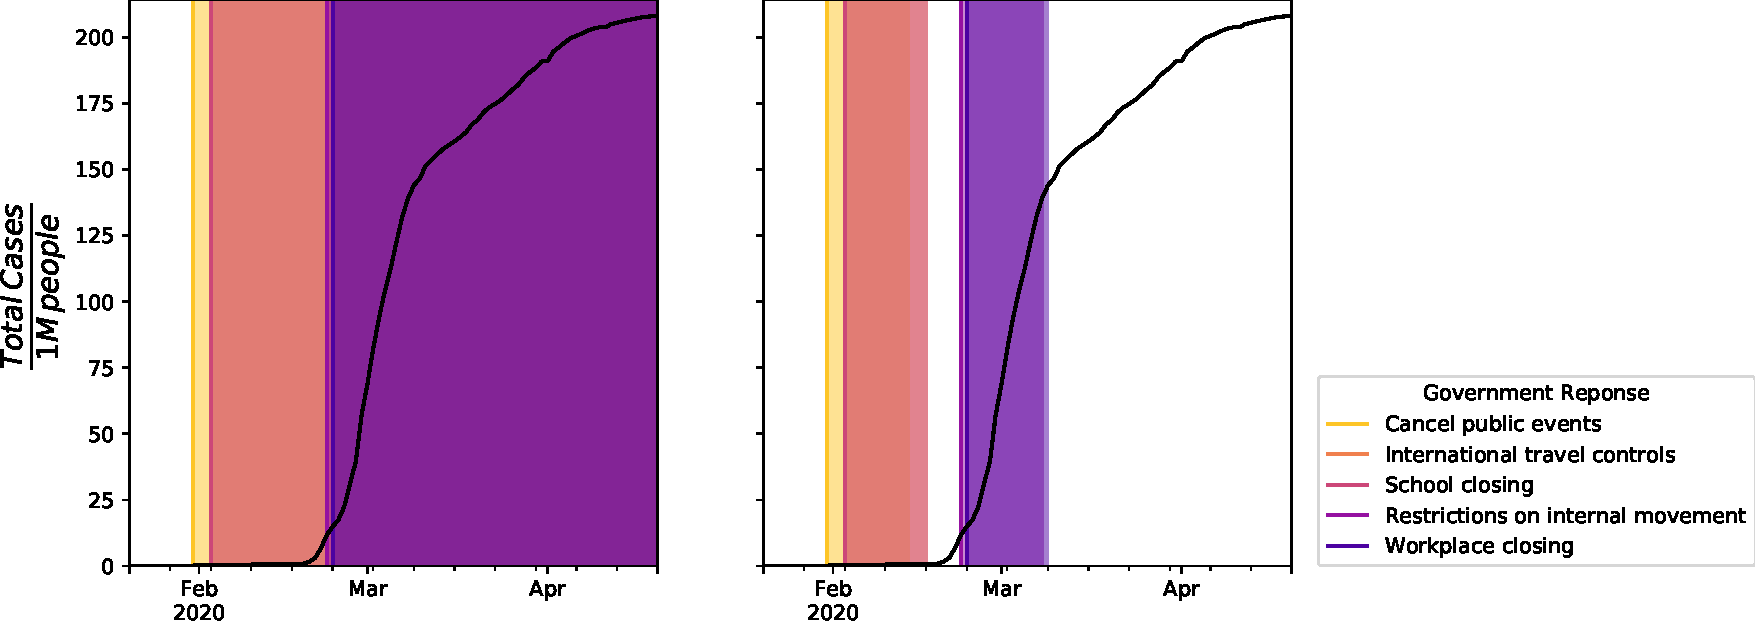
\includegraphics[width=15cm]{mg1.pdf}
\caption{The time series of the total cases per capita for South Korea. (Left) The colored rectangles indicate the active dates for each quarantine measure. (Right) The width is now a 14 day window, approximating the incubation period for COVID-19.}
\label{fig:SKrate}
\end{figure}
Figure \ref{fig:SKrate} demonstrates a time series of total cases for South Korea. The widths
of the colored regions represent different quantities; on the left it demonstrates the total amount
of time certain measures have been in effect while on the right it only shows a 14-day window
after the implementation of each measure. These 14-day windows attempt to account for the time-delayed effect resulting from incubation time. 
The claim that we are pushing is that the rate of change increased until 14 days after the strictest level of quarantine measures were introduced, implying that only then were the measures sufficient.
This behavior is incorporated directly into the analysis. For every quarantine measure, 14 day windows of the time series are taken prior and after each implementation date. The average of the total cases per capita is taken on these windows which results in a triplet of past, present, and future cases per capita values. By assuming exponential growth,
the growth rate before the quarantine measure and after as well as their difference are calculated using
\begin{align}
\rho_{i} &= \frac{1}{\Delta t_{mi}}\log(\frac{\phi_m}{\bar{\phi}_i})\nonumber \\
\rho_{f} &= \frac{1}{\Delta t_{fm}}\log(\frac{\bar{\phi}_{f}}{\phi_m})\nonumber \\
\rho &= \rho_{f}-\rho_{i} \,,
\label{eq:avgrates}
\end{align}
where over-bars denote averages over each window.
By iterating over the countries and government responses, equation (\ref{eq:avgrates}) produces a table of observations on which two-way ANOVA can be applied. Specifically,
the blocks were taken to be the different quarantine measures and the treatments were taken to be the countries. The confidence level is chosen to be 95\% and the corresponding hypothesis set can be written as
\begin{align}
    H_0 &: \mu_0 = \mu_1 = ... = \mu_a \nonumber\\
    H_1 &: \text{any of the means is different} \nonumber
\end{align}
The actual application of ANOVA was straight forward using \texttt{statsmodels} Python API. The results in table \ref{table:mganovaresults} look promising with p-values of 0.037 and 0.000003 for the choice of quarantine measure and country, respectively.

\begin{table}[ht]
\centering
\caption{Two-Way ANOVA results for change in growth rate by factor}
\label{table:mganovaresults}
\begin{tabular}{|c|c|c|c|c|}
\hline
        & Sums of squares & d.o.f. & F-stat & p-value \\ \hline
Type    & 6.757982 & 4 & 2.618791 & 0.037044 \\\hline
Country & 71.847056 & 40 & 1.8343 & 0.000003 \\
\hline
\end{tabular}
\end{table}
\begin{figure}[htb!]
  \centering
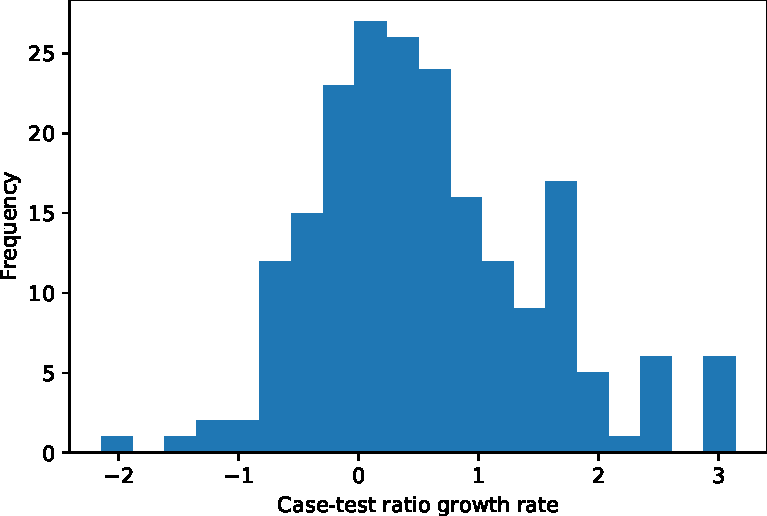
\includegraphics[width=0.4\textwidth]{mg2.pdf}\label{fig:mg2}
  \hfill
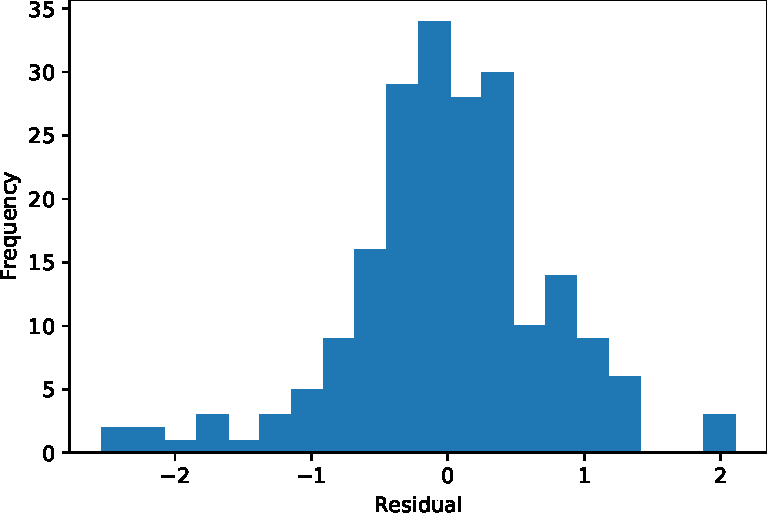
\includegraphics[width=0.4\textwidth]{mg3.pdf}\label{fig:mg3}
  \caption{Observed value and residual distributions}
    \label{TCHist}
\end{figure}
\begin{figure}[htb!]
  \centering
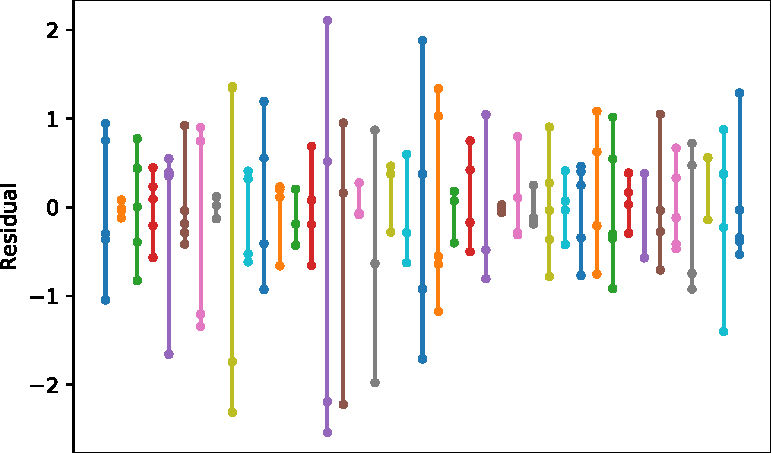
\includegraphics[width=0.4\textwidth]{mg4.pdf}\label{fig:f1}
  \hfill
  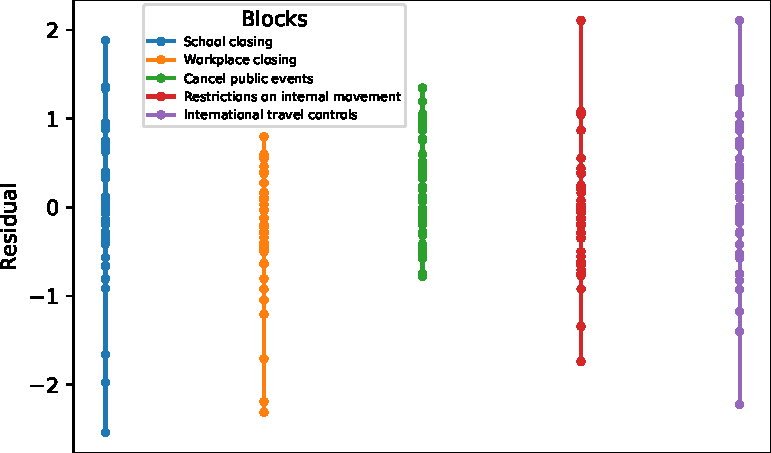
\includegraphics[width=0.4\textwidth]{mg5.pdf}\label{fig:f2}
  \caption{Variance comparisons for treatment residuals (left, countries) and block residuals (right, government responses). There are too many countries to label conveniently but the order from left to right
  is equivalent to the lexicographical ordering in the corresponding
  appendix table.}
    \label{TCvarbar}
\end{figure}
To validate these results the distribution of the observations and their residuals (Figure \ref{TCHist}) as well as variance comparison plots for countries and government responses are displayed (Figure \ref{TCvarbar}). The residuals and observations are approximately normally distributed and the variances for the blocks seem similar. The main area of concern is the variances of each countries' residuals. These disparate variances affect the interpretation of the ANOVA results; especially the effect that the countries have on the rate change. Additionally, these results may be misleading because the quarantine measures overlap with one another; when combined with the time delayed nature of the problem these results should be viewed skeptically. 



